\documentclass{article}
\usepackage[dvipsnames]{xcolor}							
\usepackage[english]{babel}
\usepackage[utf8x]{inputenc}
\usepackage[T1]{fontenc}
\usepackage{graphicx} % Required for inserting images
\usepackage{pdfpages}
\usepackage{amsmath}
\usepackage{amssymb}
\usepackage{amsthm}
\usepackage{latexsym}
\usepackage{mathtools}
% \usepackage{tikz-cd}
\usepackage{graphicx}
% \usepackage[linesnumbered,ruled,vlined,algo2e]{algorithm2e}
\usepackage[margin=1in]{geometry}
\usepackage{hyperref}
\usepackage{cleveref}
\usepackage{caption}
% \textheight=700px                    % Saving trees ;-)
\frenchspacing 
\hypersetup{
    pagebackref=true,
    colorlinks = true,
    allcolors = OliveGreen}

\def\minpts{\operatorname{MinPts}}
\def\R{\mathbb{R}}
\def\Z{\mathbb{Z}}
\newtheorem{definition}{Definition}[section]
\newtheorem{example}{Example}[section]
\newtheorem{remark}{Remark}[]
\newcommand{\comment}[1]{{\color{violet} \it #1}}

\title{TDA24 - Mapper}
\author{}
\date{}

\begin{document}

\maketitle

\section{Introduction [Project Statement]}

The mapper algorithm is a popular tool for visualization and data exploration in topological data analysis. The recent paper \textit{Any graph is a Mapper graph} \cite{alvarado2024graphmappergraph} investigates an inverse problem for the mapper algorithm: \linebreak
Given a dataset $X$ and a graph $G$, does there exist a set of mapper parameters such that the output mapper graph of $X$ is isomorphic to $G$? Two constructions are provided that affirmatively answer this question. Some natural follow-up questions are:
\begin{itemize}
    \item What are some other constructions?
    \item What are some constructions when we add constraints, e.g. reference space is $\R$, or fix the clustering function?    
    \item Is there anything we can say about ``how big'' the set of mapper parameters that work for a particular graph and dataset? 
    \item For the construction that maps into convex sets in $\R^3$, what map allows for the largest extension?
    \item Write code that constructs convex sets in $\R^3$ whose nerve is $G$; starting with subsets of $\R^4$ is easier.
    \end{itemize}

\subsection{Ideas}

Simplex Tree \cite{simplex-tree-Boissonnat_2014}.

Any graph is indeed a mapper graph \cite{alvarado2024graphmappergraph}, however, in their mapper construction, they only use a trivial clustering function. Can these results be shown when considering other clustering functions such as \underline{DBSCAN} \cite{DBSCAN} or a \underline{neighborhood graph clusterer}?

Is there an example with a "regular cover" where you cannot construct a mapper graph isomorphic to a graph? 
Is there a map from a regular mapper cover (intervals of different lengths and overlaps but no redundant cover sets to a more regular mapper cover (same interval lengths and gain)

We need to make a metric to compare mapper graphs! We can compare functions to one another and cover sets. We should think of graph metrics. See Section \ref{sec:graph-metrics}

\section{Notes on DBSCAN [Halley]}

\subsection{BIG DBSCAN RESULTS FOR MAPPER}
This paper posted on the arxiv in September giving some related results on how DBSCAN effects Mapper.
\href{https://arxiv.org/pdf/2409.17360}{Bifiltration and Stability of TDA Mapper for point cloud data}.

\subsection{DBSCAN Notes.}

Let $(X,d)$ be a data set we wish to cluster with metric $d$. Choose parameters $\varepsilon>0$ and positive integer $\minpts\in\Z_+$.

\begin{definition}[$\varepsilon$-neighborhood]
    For point $p\in X$ we define the \underline{$\varepsilon$-neighborhood of $p$} as 
    $$N_\varepsilon(p)=\{q\in X | d(p,q)<\varepsilon\}.$$
    If $|N_\varepsilon(p)|\geq \minpts$ we call $p$ a \underline{core point}, otherwise $p$ is a \underline{border point}.
\end{definition}
\begin{definition}[density reachable]
    For $p,q\in X$ we say that $p$ is \underline{directly density reachable} from $q$ if $p\in N_\varepsilon(q)$ and $q$ is a core point.
    
    \noindent A point $p$ is \underline{density reachable} from $q$ if there exists a chain of points $p_1,...,p_n$ such that $p_1=q, p_n=p$ and $p{i+1}$ is directly reachable from $p_i$ for all $1\leq i\leq n$.
\end{definition}
Density reachability is not symmetric in general but it is transitive.

\begin{definition}[density connected]
    A point $p$ is \underline{density connected} to a point $q$ if there exists point $w$ such that both $p$ and $q$ are density reachable from $w$.
\end{definition}
\begin{definition}[cluster]
    For a data set $X$, a \underline{cluster} of points $C$ is a non-empty subset of $X$ such that for all $p,q\in C$
    \begin{itemize}
        \item[(Maximality) $\circ$] if $p\in C$ and $q$ is density reachable from $p$ then $q\in C$
        \item[(Connected) $\circ$] $p$ is density connected to $q$
    \end{itemize}
    A point $q\in X$ is called \underline{noise} if $q\notin C_i$ for all $i$. Let $N$ denote the set of all noisy points.
\end{definition}

\subsection{DBSCAN Algorithm}

\begin{enumerate}
    \item Choose random point $p\in X$
    \item Find all points in $X$ that are density reachable from $p$ and call this set $S$.
    \begin{itemize}
        \item If $p$ is a core point, $S$ is a cluster.
        \item If $p$ is a border point, $S=\emptyset$. Continue to the next point in $X$.
    \end{itemize}
    \item Let $S_1,S_2$ be two such sets for points $p_1,p_2$ respectively. Define $d(S_1,S_2)=\min\{d(p,q) | p\in S_1, q\in S_2\}$. If $d(S_1,S_2)>\varepsilon$, then $S_1$ and $S_2$ are two distinct clusters and we label them $C_1$ and $C_2$.
\end{enumerate}
This separates $X$ into clusters where each cluster $C_i$ contains at least $\minpts$ many points. Border points in $X$ are considered noise, so this gives us a decomposition of our dataset $X=\bigcup_i C_i \cup N$. 
Something to note about mapper is that if a point is considered noise during the clustering, then it should become its own node in the graph. \comment{We should double-check this.}

\subsubsection{Heuristic for determining parameters}
See \cite[Section 4.2]{DBSCAN} (\url{https://www.dbs.ifi.lmu.de/Publikationen/Papers/KDD-96.final.frame.pdf}) for their method. They only applied this heuristic for two-dimensional data.
\section{Triangle data coding [Nick and Aine]}

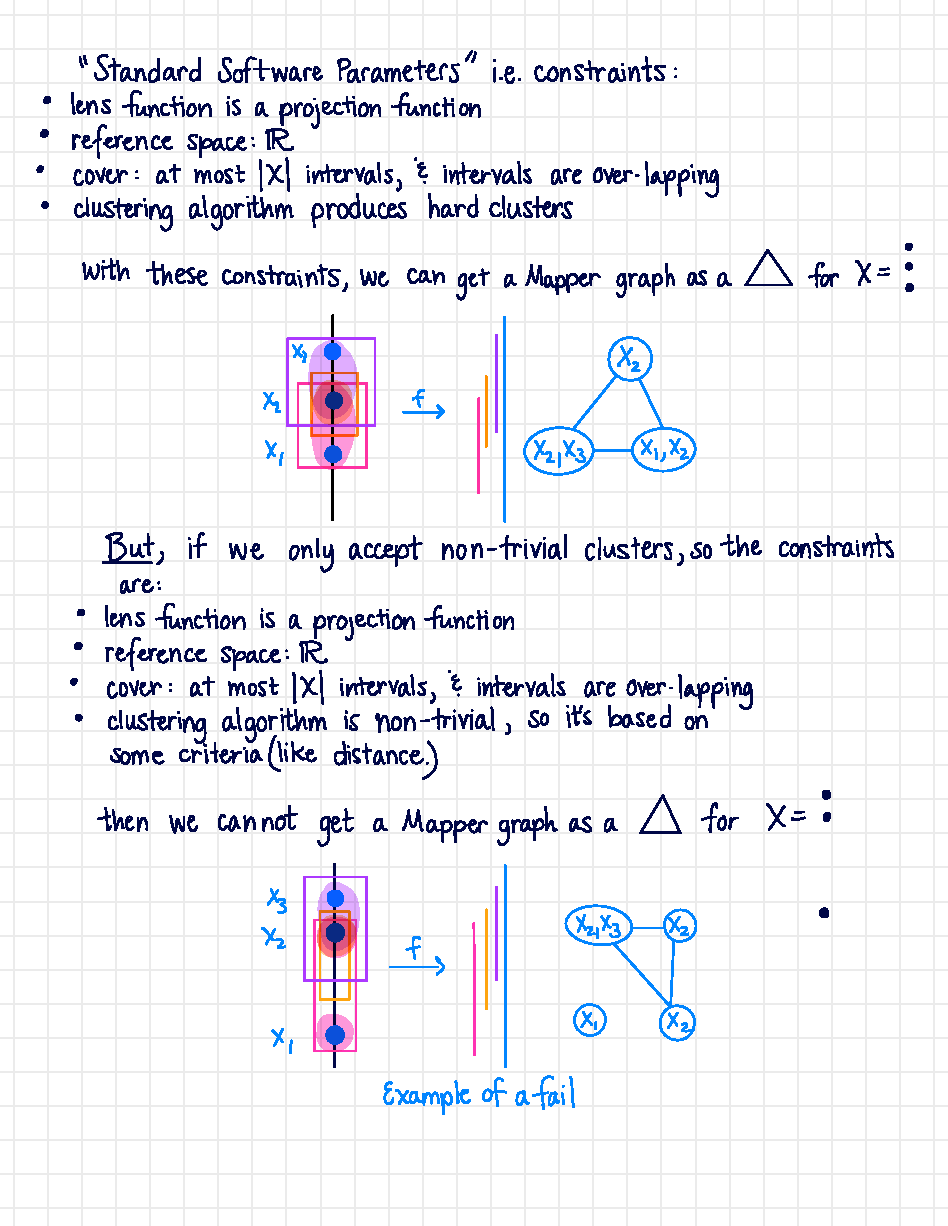
\includegraphics[]{Example.pdf}
\subsection{code}
colab notebook: \url{https://colab.research.google.com/drive/13EMEqqkLah7QhznlMKGHGWRAHyr1SwS5?usp=sharing}
\subsection{notes and observations}
For both DBSCAN and k-means, there are conditions in which generating three points will generate a triangle graph, but for both the overlap is excessively high. For KMeans, to reliable receive a triangle from data points the overlap between intervals has to be greater than 0.999. Finding a lower overlap may have to look at it as a function of not only the distance of the far point from the two close ones, but also how close the close points are (?). A similar pattern exists for DBSCAN. 
\subsection{future directions}

\section{Notes on Graph Metrics [Halley]}\label{sec:graph-metrics}
We talked about considering graph metrics for comparing individual mapper graphs. In particular the survey of graph metrics by Erin Chambers, et al. \cite{Buchin2023-graph-metrics} was brought up.
Below are some notes about said paper 

\url{https://link.springer.com/article/10.1007/s44007-022-00037-8}

Ones to note:
\begin{itemize}
    \item Local Persistent Homology Distance (3.9)
    \item Hausdorff Distance (3.1)
    \item Graph Edit Distance (3.8)
\end{itemize}

\subsection{Hausdorff Distance}
\subsection{Local Persistent Homology Distance}

Given a metric space $(M,\delta)$, let $\mathcal{G}_M$ be the collection of finite graphs immersed in $M$. Each $(G,\phi)\in\mathcal{G}_M$ is a graph $G=(V,E)$ of vertices $V$ and edges $E$ with an immersion $\phi\colon G\to M$.

\begin{definition}[Bottleneck Distance]
    Let $D_1$, $D_2$ be two persistence diagrams. The \underline{bottleneck distance} $d_b$ is defined as 
    $$ d_b(D_1,D_2) := \inf_{f\colon D_1\to D_2}\sup_{x\in D_1} ||x-f(x)||,$$
    where $f$ ranges over all bijections between $D_1$ and $D_2$.   
\end{definition}
The Local Persistent Homology Distance compares graphs at a local level. Let $\mathbb{Y}\subseteq \mathbb{X}$ be a set. We define the \underline{$\varepsilon$-thickening} of $\mathbb{Y}$ to be
    $$ \mathbb{Y}^\varepsilon := \bigcup_{x\in\mathbb{Y}}B_d(x,\varepsilon) = \{x\in \mathbb{X}\colon d(\mathbb{Y},x)\leq\varepsilon\}.$$

Let $(G,\phi_G)\in\mathcal{G}_M$, and define the function $\delta_G\colon M\to\R$ as the distance function to the set $\phi_G(G)$, defined $\delta_G(x):=\min_{y\in\phi_G(G)}\delta(x,y)$ for all $x\in M$. Equivalently, $\delta_G(x)$ is the smallest non-negative $\epsilon$ such that $x\in G^\epsilon$. For closed subsets $U\subseteq M$ define $\delta_{G,U}\colon U/\partial U\to \R$ by 

\begin{equation}
\delta_{G,U}([x])=\left\{
\begin{aligned}
&\delta_G(x),\quad &[x]\neq\partial U,\\
&\min_{y\in\partial U}\delta_G(y), &[x]=\partial U.
\end{aligned}\right.
\end{equation}

For graphs $(G_1,\phi_1)$ and $(G_2,\phi_2)$ in $\mathcal{G}_M$, let $D_1$ and $D_2$ be persistence diagrams of $\delta_{G_1,U}$ resp. $\delta_{G_2,U}$. Let $B_U(G_1,G_2)$ denote the \textit{local distance signature} between $G_1$ and $G_2$ to the closed set $U$.

\subsection{Additional Papers for Metrics}
Erin Chambers, et al \cite{bollen2022reebgraphmetricsground} have an extensive paper on metric for Reeb Graphs. I am unsure if any of these will generalize for applications nicely. Additionally, Erin mentioned a recent Bei Wang paper \cite{mapper-AI-activations} which actively compares mapper graphs for activation layers of convolutional neural networks. 

\section{Mapper comparison with optimal transport}
Notes from the Bei Want paper comparing mapper graphs for activation layers of convolutional neural networks. 
Each mapper graph is hepergraph in which each data point is a vertex in the hypergraph and a cluster of data points from the mapper graph forms a hyper edge. We treat each hypergraph as a measure hypernetwork using existing tools from optimal transport \href{https://arxiv.org/pdf/2112.03904}{(see the following preprint)}.

\begin{definition}
    A \underline{measure hypernetwork} is a tuple $\mathcal{H}=(X,\mu,Y,\nu,\omega)$, where $X$ and $Y$ are well-behaved topological spaces (Polish spaces), $\mu,\nu$ are probability measures on $X$ and $Y$ and $\omega\colon X\times Y\to \R$ is a measurable and bounded weight functions that captures the relations between elements in $X$ and $Y$.
\end{definition}

We treat the mapper graph as a finite hypergraph $H=(X,Y)$, where $X$ is the set of vertices, an $Y$ is a set of hyperedges. We can model $H$ as a hypernetwork $\mathcal{H}$ by introducing probability measures $\mu, \nu$ based on the structure of $H$ and the weight function $\omega$ based on the node-hyperedge relations (see \cite[Figure 4]{mapper-AI-activations}). For a more interesting $\omega$ we may define $\omega$ as the \emph{shortest path distance} where $H$ is a weighted hypergraph with weights determined by the 1/Jaccard index of two hyperedges.

Given two hypernetworks $\mathcal{H}, \mathcal{H}'$ modeling mapper graphs, the Gromov-Wasserstein distance between them as defined \href{https://arxiv.org/pdf/2112.03904}{here}
$$ d_{GW}(\mathcal{H},\mathcal{H}')^2=\min_{\pi\in C(\mu,\mu'),\xi\in C(\nu,\nu')}
\left(\sum_{x\in X, y\in Y, x'\in X', y'\in Y'} 
(\omega(x,y)-\omega'(x,y))^2
\pi(x,x')\xi(y,y')
\right)$$
where $\pi$ is a coupling (joint probability measure) $X$ and $X'$ such that its marginal agree with $\mu$ resp $\mu'$. $C(\mu,\mu')$ is the set of couplings between $\mu$, $\mu'$ (Similar definitions for Y).

To actually compute any Gromov-Wasserstein distances between mapper graphs they use the \href{https://arxiv.org/pdf/2002.03731}{Co-Optimal Transport} after initializing the coupling matrices $\pi$, $\xi$. They initialize $\xi$ and $\pi$ as follows: randomly generate elements in $\xi$ via a gamma distribution and then apply a \href{https://arxiv.org/pdf/1306.0895}{Sinkhorn optimization} to ensure the marginal distributions of the couplings are consistent with the hyperedges of $\nu$ and $\nu'$ (similarly for $\pi$).


\bibliographystyle{plain}
\bibliography{main}

\end{document}
